% build with: pdflatex --shell-escape fig.tex
\documentclass[tikz, convert={density=800}]{standalone}

\usepackage{tikz}
\definecolor{myOrange}{HTML}{ffa500}
\definecolor{myBlue}{HTML}{42affa}

\begin{document}
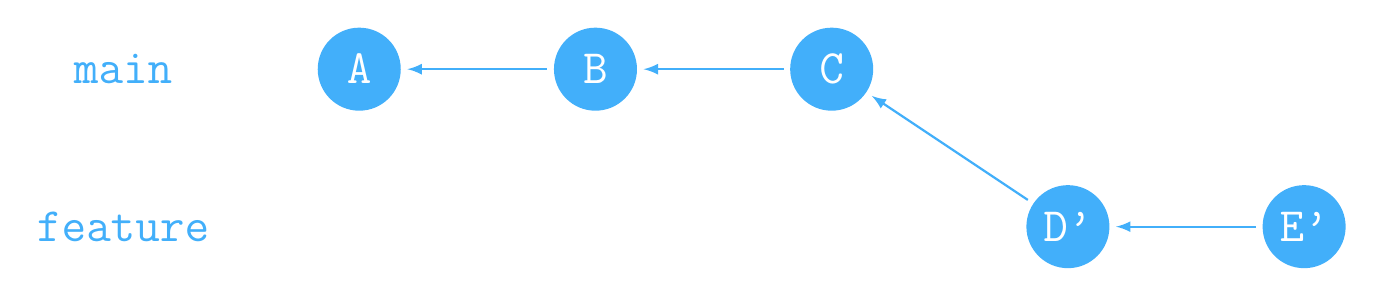
\begin{tikzpicture}[>=latex, thick, shorten >=2pt, shorten <=2pt, ->, myBlue]
  \tikzstyle{C}=[circle,fill=myBlue,text=white,minimum size=30pt,inner sep=2pt, font=\LARGE]
  \tikzstyle{M}=[circle,fill=myOrange,text=white,minimum size=30pt,inner sep=2pt, font=\LARGE]
  \tikzstyle{B}=[text=myBlue, font=\LARGE]

  \node[C] at (0,3) (A) {\texttt{A}};
  \node[C] at (3,3) (B) {\texttt{B}};
  \node[C] at (6,3) (C) {\texttt{C}};
  
  \node[C] at (9,1) (D) {\texttt{D'}};
  \node[C] at (12,1) (E) {\texttt{E'}};

  \draw [<-] (A) to (B);
  \draw [<-] (B) to (C);
  \draw [<-] (C) to (D);
  \draw [<-] (D) to (E);
  
  \node[B] at (-3,3) {\texttt{main}};
  \node[B] at (-3,1) {\texttt{feature}};
  
\end{tikzpicture}
\end{document}
